\chapter*{Introduction}\addcontentsline{toc}{chapter}{Introduction}\markboth{Introduction}{Introduction}

In the Czech timber industry, logs are typically cut according to predefined patterns without regard for internal structure. This approach leads to suboptimal lumber yields, because flaws such as knots, cracks, and rot remain concealed inside the log and are not identified until after processing. Computed tomography (CT) offers a way to reveal these internal defects, allowing sawmills to produce better-quality planks, increasing economic returns. However, no publicly available CT dataset of logs with voxel-level defect annotations that conforms to Czech technical standards exists.

A dataset of 40 CT-scanned oak logs provided by the Czech University of Life Sciences in Prague is used to address this gap. A substantial portion of the work is devoted to the annotation of defects within this dataset, which forms the basis for subsequent analysis and modeling. The annotated data are then used to develop and evaluate methods for detecting and classifying defects within the 3D structure of the logs.

The primary goal is to create a CT dataset of oak logs with defect categories defined according to industry standards. Furthermore, the thesis aims to develop and evaluate algorithms capable of reliably detecting and classifying defects within the 3D volume of a log. The results are intended to serve as the foundation for a system that optimizes cutting strategies and improves the economic efficiency of wood processing in the Czech Republic.

\setcounter{page}{1}


\chapter{Research}
\label{chap:research}
CT-based analysis of wood defects involves challenges in volumetric data processing, segmentation, and working with limited annotated data. Therefore, existing research was examined to identify effective preprocessing strategies, suitable model architectures, and common limitations. In parallel, available datasets were reviewed to determine whether a suitable resource for CT-based wood defect analysis already exists or whether the creation of a new dataset is necessary.



% ---------------------------------------------------------------
\section{Overview of Related Work}
% ---------------------------------------------------------------

A foundational study~\cite{Schmoldt_1998} reviews the lumber extraction process and evaluates various generations of CT scanning technologies. To automate defect detection, the authors employed a feed-forward back-propagation neural network that classified each non-background pixel based on its local neighborhood. The model used a 2D ($5 \times 5$) and a 3D ($3 \times 3 \times 3$) feature window achieving high precision, with more than 95\,\% for the classification of a single species and approximately 91–92\,\% for multiple species using 10 fold cross-validation. An important finding was that 3D feature windows outperformed 2D windows when generalizing across different wood species, highlighting the importance of inter-slice information for reliable defect detection.

\begin{figure}[H]
    \centering
    \includegraphics[width=0.75\textwidth]{images/schmoldt_ann.png}
    \caption{The neural network used for log defect segmentation. The network classifies the center pixel by taking the normalized pixel values of the surrounding feature window and the pixel's radial distance from the pith as inputs.~\cite{Schmoldt_1998}}
    \label{fig:schmoldt_ann}
\end{figure}

In~\cite{gergel2026wood} a dataset of three oak log sections was used, producing a total of 380 annotated CT images. Furthermore, two architectures were utilized: DeepLab~v3+~\cite{chen2018deeplabv3plus} with a ResNet-50~\cite{he2016resnet} backbone for semantic segmentation of wood, bark and background. Inception-v3~\cite{szegedy2016rethinking} was used for the binary classification of the presence of defects. Data augmentation techniques, including random rotations and horizontal/vertical flips, were applied. For bark segmentation, the DeepLab~v3+ network achieved Dice coefficients of 0.9814 for wood, 0.7502 for bark after postprocessing and 0.9976 for outskirts. The authors found that bark was the most challenging class due to its irregular geometry and low contrast at the log boundary and showed that enriching the training set with manually selected difficult cases improved the bark Dice score from 0.558 to 0.7502.

\begin{figure}[H]
    \centering
    \begin{subfigure}[b]{0.48\textwidth} 
        \centering
        \includegraphics[width=\textwidth]{images/rgb_prior.png}
        \caption{Three adjacent grayscale CT slices.}
        \label{fig:gray_slices}
    \end{subfigure}
    \hfill
    \begin{subfigure}[b]{0.48\textwidth} % Scaled down slightly
        \centering
        \includegraphics[width=\textwidth]{images/rgb.png}
        \caption{The slices mapped to RGB channels.}
        \label{fig:rgb_slices}
    \end{subfigure}
    
    \caption{A pseudo 3D representation achieved by combining consecutive 2D slices into an RGB image.~\cite{khazem2023deep}}
    \label{fig:rgb_slice_stacking}
\end{figure}

To implement a limited 3D context, the authors adopted an RGB representation in which three adjacent grayscale CT slices were combined into a single image by mapping each slice to one of the three color channels. This strategy increased classification accuracy from  93.94\% to 95.39\%, but remains only a simplification of true 3D information. The authors acknowledged that this is fundamentally an approximation of three-dimensional data and suggested that native 3D
convolutional networks offer a more principled direction for future work.

Another approach presented by~\cite{khazem2023deep} analyzes CT scans of wood logs using a ResNet-34 regression model for pith detection, along with a U-Net for contour extraction and knot segmentation. The study was conducted on a diverse dataset comprising 682 trees of 23 species. For knot segmentation, the U-Net achieved a Dice score of 0.698 when trained on 2,504 annotated images with data augmentation and demonstrated the ability to generalize to previously unseen species. However, this approach utilized each CT slice separately and therefore did not take advantage of the full 3D spatial context. The authors highlighted that convolutional networks struggle with representing intricate knot configurations and proposed the use of self-attention blocks. This motivates the adoption of transformer architecture, such as SwinUNETR, which operates directly on 3D volumes using self-attention to model complex spatial relationships more effectively. 

A detection workflow proposed by~\cite{xie2026deep} outlines a 3D reconstruction approach for internal wood defects, specifically decay, hollows, and knots, using CT imaging data. They proposed SCV-YOLOv8n, a modified segmentation framework derived from YOLOv8n-seg~\cite{yolov8_ultralytics}, designed to enhance feature extraction and increase segmentation robustness when dealing with irregular defect boundaries and complex textural patterns. To map the resulting 2D segmentation masks into a 3D volumetric representation, the standard Visualization Toolkit pipeline was extended with additional submodules to enforce internal consistency and achieve a more coherent transition from 2D segmentations to 3D volumes.


In the Medical Segmentation
Decathlon~\cite{antonelli2022msd}, the participants were
tasked with creating a general algorithm capable of segmenting ten different
datasets covering a range of organs. The datasets posed several difficulties,
including very limited training data,
severe class imbalance, and small or irregular targets.

U-Net was the most popular base architecture, chosen by 64\% of the
participating teams. Furthermore, the best performing methods shared the use of Dice loss and data augmentation. The
winning method, nnU-Net~\cite{antonelli2022msd, isensee2021nnunet},
demonstrated that preprocessing, architecture
topology, and a training strategy optimized to the properties of each dataset were more impactful than the novel architectural design.


\section{Review of Datasets}
Since the studies outlined above depend on private wood CT scan datasets, this thesis instead examines alternatives.

The Swedish Stem Bank~\cite{grundberg1995ssb} contains CT scans for several hundred logs. Although not public, researchers can obtain access on request. However, instead of detailed voxel-level annotations, internal defects such as knots are described using mathematical descriptors such as the vertical position of the knot, the radial angle, and the distance from the base. Because modern deep learning segmentation models depend on precise and dense spatial masks to capture the true shapes of natural defects, the absence of such accurate annotations greatly restricts the usefulness of the dataset for training modern 3D networks.


A recent dataset~\cite{lulea2025resinwood} contains
high-resolution industrial CT scans with a voxel size of approximately
0.3~mm. However, the annotations in this dataset are limited to
areas associated with a specific fungal infection (\textit{Cronartium pini}). Due to this narrow focus, the dataset is not suitable for general defect detection.

\begin{figure}[htbp]
    \centering
    \includegraphics[width=0.9\textwidth]{FITthesis-LaTeX-master/images/wood_surface.png}
    \caption{Visualization of a 2D surface defect dataset. Visible defects include knots (green), rot (red), resin pockets (pink), and knots with cracks (orange).~\cite{kodytek_pavel}}
    \label{fig:2d_dataset_example}
\end{figure}


Another dataset~\cite{kodytek_pavel} consists of 2D images of wood that contain more than
43,000 annotated defects, including knots, cracks, and resin pockets.
The dataset is based on standard camera images rather than CT scans, making it fairly limited in modern 3D model approaches.

\chapter{Theoretical Background}

The fundamentals of CT imaging and volumetric data representation, rooted in techniques widely used in the medical field, are introduced first, followed by the model architectures used for segmentation. The chapter concludes with the segmentation formats relevant for defect modeling.

\section{DICOM Overview}

The experimental dataset provided by the Faculty of Forestry and Wood Science
of the Czech University of Life Sciences (CZU) consists of CT scans created by a Siemens Somatom Scope Power CT scanner. The system
outputs imaging data in the proprietary \texttt{.IMA} file format. These files
are fully compliant with the Digital Imaging and
Communications in Medicine (DICOM) standard, which serves as the universal protocol
for the transmission and storage of medical imaging information~\cite{dicom_standard}.

\subsection{Principles of Computed Tomography}

Computed tomography is an imaging technique that uses an X-ray source
mounted on a rotating gantry opposite a detector array~\cite{bushberg2011essential}. Unlike standard 2D
radiography, which captures a single static projection, the CT gantry rotates
around the object to acquire X-ray attenuation profiles
from thousands of distinct angular positions.

\begin{figure}[H]
 \centering
 \includegraphics[width=0.5\textwidth]{images/ct_scanner_geometry.png}
 \caption{Illustration of a third-generation CT scanner. The X-ray source and the detector array rotate simultaneously around the object to capture attenuation profiles from multiple angles.~\cite{Schmoldt_1998}.}
 \label{fig:ct_generation}
\end{figure}

These raw attenuation profiles are mathematically processed using
reconstruction algorithms to generate
tomographic images. These images represent virtual slices of the object's
internal structure perpendicular to the scan axis.~\cite{Schmoldt_1998}

\subsection{The Hounsfield Unit}

The CT scanner relies on the principles of X-ray attenuation. As the X-ray
beam passes through the oak log, its intensity decreases depending on the
density and composition of the material. This exponential drop in intensity is
described by the Beer--Lambert Law~\cite{bushberg2011essential}:

\begin{equation}
 I = I_0 \, e^{-\mu x}
 \label{eq:beer_lambert}
\end{equation}

\noindent where $I_0$ is the initial intensity of the X-ray beam, $I$ is the
 intensity detected after passing through the object, $x$ is the thickness of
the material, and $\mu$ is the linear attenuation coefficient.

During the scanning process, the CT hardware measures the transmitted intensity
($I$) across a known path length ($x$) given the known initial intensity
($I_0$). By recording these values from thousands of angles, the system solves for the linear attenuation coefficient ($\mu$)
in every voxel  (volumetric
pixel).

However, because the absolute value of $\mu$ depends on the energy of the
X-ray beam, the raw attenuation values are not directly comparable
between different scans. Therefore, these values are standardized onto the
Hounsfield Scale~\cite{hounsfield1973computerized}, which normalizes the attenuation of a material against that
of distilled water.

\begin{equation}
 HU = 1000 \times
 \frac{\mu_{\text{material}} - \mu_{\text{water}}}
{\mu_{\text{water}} - \mu_{\text{air}}}
 \label{eq:hu_definition}
\end{equation}

By definition, distilled water is calibrated to 0~HU and air to $-1000$~HU. In
the context of oak logs, this scale provides a high contrast between low-density
defects such as cracks or rot, which approach $-1000$~HU and high-density
features such as healthy wood, ranging from approximately $-600$ to $+500$~HU,
and knots, which usually range from $+300$~HU to $+600$~HU depending on species and moisture~\cite{freyburger2009measuring}.

\subsection{DICOM Structure and Data Encoding}

The \texttt{.IMA} DICOM files act as containers that encapsulate two distinct
data components: a metadata header comprising information such as exposure
time and spatial resolution, and the associated raw pixel data.

When stacked sequentially, these 2D slices form a volumetric representation of
the log. The fundamental unit of this 3D volume is the voxel. Unlike a 2D pixel, which encodes a value at coordinates $(x, y)$, a
voxel encodes a value at a position on a regular three-dimensional grid 
$(x, y, z)$. The depth of the voxel is determined by the thickness of the slice, while its dimensions in the xy plane are defined by the pixel spacing.

The raw pixel data within the Siemens \texttt{.IMA} files are stored as
unsigned 16-bit integers. However, because Hounsfield Units can be negative
(e.g.\ air at $-1000$~HU), the stored integer values ($P_{\text{raw}}$) must
be transformed using a linear equation defined in the DICOM header~\cite{dicom_standard}:

\begin{equation}
    HU = (P_{\text{raw}} \times \text{RescaleSlope}) + \text{RescaleIntercept}
    \label{eq:dicom_conversion}
\end{equation}

\noindent where \text{RescaleSlope} and \text{RescaleIntercept} are parameters specific to individual scanners. For the Siemens Somatom system used in this study, the slope is 1 and the intercept is $-1024$. Consequently, a raw integer value stored in $0$ corresponds directly to $-1024$~HU.

Once the pixel values are converted to the Hounsfield scale, a windowing operation is performed. This technique narrows the wide dynamic range of the CT  to the specific HU band relevant to wood and its structural defects. By excluding irrelevant density extremes, the volumetric dataset is refined for more efficient processing.~\cite{dicom_standard}


\section{Segmentation Architectures}
Several segmentation architectures, ranging from traditional convolutional networks to transformer based methods, are described below.

\subsection{U-Net}

The U-Net architecture, originally proposed by ~\cite{ronneberger2015unet}, is made up of two symmetric branches: an encoder and a decoder. The
encoder gradually decreases the spatial resolution of the input while learning
progressively more abstract feature representations. The decoder gradually
restores the spatial resolution, enabling accurate localization by projecting features back onto the pixel grid.

A key feature of U-Net is its use of skip connections, which
concatenate the feature maps from each encoder level with those of the
corresponding decoder level. This mechanism enables the network to fuse
spatial detail with rich semantic information from deeper
layers. Consequently, U-Net is particularly effective in segmenting fine
structures, such as cracks and insect damage, in CT images.

The decoder reconstructs the spatial resolution using up-convolution
operations, typically implemented as transposed convolutions. These layers
perform learnable upsampling by increasing the spatial dimensions of the
feature maps, allowing the network to recover fine structural details lost
during downsampling. At each decoding stage, the upsampled feature maps are
concatenated with the corresponding encoder features via skip connections,
followed by convolutional refinement. This iterative process enables the
network to progressively reconstruct a dense segmentation map that is both
spatially precise and semantically consistent.

\begin{figure}[H]
    \centering
    \includegraphics[width=0.9\textwidth]{images/u-net-architecture.png}
    \caption{The standard U-Net architecture, featuring a symmetric encoder--decoder structure with skip connections.~\cite{ronneberger2015unet}}
    \label{fig:unet}
\end{figure}


\subsection{nnU-Net}
% ---------------------------------------------------------------
The performance of U-Net architectures is highly dependent on design choices such as patch size, batch size, normalization scheme, and data augmentation strategy. To systematically address this sensitivity, the \textit{no-new-Net} (nnU-Net) framework introduced in~\cite{isensee2021nnunet} offers a deterministic configuration pipeline driven entirely by the properties of the dataset.

nnU-Net supports three main configurations:

\begin{itemize}
    \item \textbf{2D U-Net} operates on individual slices independently.
    \item \textbf{3D full-resolution U-Net} processes patches extracted from the full 3D volume.
    \item \textbf{3D Cascade} is a two-stage pipeline where a low-resolution 3D U-Net first produces coarse segmentations, which are subsequently refined by a second full-resolution network at full detail.
\end{itemize}

All three configurations were considered for this work. The choice between them is made empirically per dataset, and the comparison for the oak log volumes is presented in the Model Selection section of the Analysis chapter.


\subsection{SwinUNETR}

SwinUNETR, introduced by ~\cite{hatamizadeh2022swinunetr}, is a hybrid segmentation model that
extends the classical U-Net design by incorporating transformer-based
representation learning into its encoder. Although the decoder largely retains
the convolutional structure of U-Net, the encoder is fundamentally redesigned
using the Swin Transformer~\cite{liu2021swin}.

This redesign directly addresses a major shortcoming of standard CNNs. Although
CNNs are effective at capturing local spatial structures, their inherently
limited receptive fields restrict their ability to model deep dependencies. This becomes particularly problematic in volumetric analysis,
where a global spatial context is often essential for accurate segmentation.

In SwinUNETR, the encoder operates on volumetric inputs by initially dividing
the input into distinct patches, which are then linearly embedded into a
sequence of feature tokens. These tokens are passed through multiple stages composed of Swin Transformer blocks. Between stages, patch
merging progressively decreases spatial resolution while increasing feature
dimensionality, supporting feature extraction.

\begin{figure}[H]
    \centering
    \includegraphics[width=\textwidth]{FITthesis-LaTeX-master/images/swinUneTrWIndows.png}
    \caption{Illustration of the 3D shifted window self-attention mechanism used in SwinUNETR. The input volume is split into a grid of 3D tokens. In Layer $l$, self-attention is computed within exclusive 3D windows. In the next Layer $l+1$, the window partitioning is  shifted, allowing information to mix across the window boundaries. Adapted from~\cite{hatamizadeh2022swinunetr}.}
    \label{fig:swinunetr}
\end{figure}

A key ability of the Swin Transformer is its efficient self-attention mechanism. Rather than computing self-attention over the entire volume, which is computationally expensive, the feature map is partitioned into groups of local windows. Self-attention is then computed independently within each window, and in subsequent layers these windows are shifted, enabling information exchange across neighboring regions. By alternating between these two operations, the model is able to capture both local structure and broader spatial context while maintaining computational efficiency.

The structure of the encoder aligns well with the design of the U-Net decoder. Features extracted at different resolutions are
passed through skip connections to the corresponding decoder stages, improving spatial localization and supporting more precise segmentation.

\subsection{MedNeXt}
MedNeXt, proposed by~\cite{roy2023mednext}, bridges the gap between traditional convolutional networks and transformer-based models. Whereas transformer architectures such as SwinUNETR excel at modeling global dependencies, they typically require large datasets to understand complex relationships. MedNeXt addresses this by preserving the strong inductive bias of convolutions while adopting architectural ideas inspired by Transformer designs.

At its core, MedNeXt follows a U-Net encoder–decoder structure, replacing standard convolutional blocks with ConvNeXt~\cite{woo2023convnextv2} building blocks. These consist of a depthwise convolution, a channel expansion layer, and a projection layer that compresses features back to the original dimensionality.

A key design choice is the use of large kernel convolutions to approximate the broad receptive fields typically associated with self-attention. To make large kernels easier to optimize in data-scarce regimes, MedNeXt leverages initialization strategies that transfer or interpolate weights from smaller kernel counterparts.

The architecture also adapts these design principles to both downsampling and upsampling routes, helping to preserve semantic information across resolutions which improves segmentation of densely packed defects.

Another important component is compound scaling. Because the architecture decouples the receptive field from network width, the number of channels, layers, and kernel sizes can be scaled simultaneously for optimal performance across different dataset sizes.

In general, MedNeXt provides a strong alternative to classical U-Net variants and transformer based models, combining convolutional efficiency and inductive bias with improved receptive field modeling and achieving strong performance on medical image segmentation tasks.


\chapter{Annotation}
\label{chap:dataset_annotation}
The dataset of CT scanned oak logs used in this work was collected by CZU and consists of 40 oak logs, each captured as a 3D volume composed of individual CT slices. Due to the absence of ground truth annotations, defect labeling and training data preparation form a substantial part of this work.

\section{Format Selection}

A fundamental design decision in constructing a segmentation dataset is the
choice of annotation format. Three relevant methods were considered: instance
segmentation, panoptic segmentation, and semantic segmentation.

Instance segmentation treats every defect as a separate object, assigning an
individual mask to each occurrence, while panoptic segmentation further
augments this with class-level labels to deliver the most complete
representation of a scene. Both approaches share a common drawback: they
impose a substantially higher annotation burden, since every object instance
must be delineated independently. This is further complicated by the difficulty
of defining clear boundaries between two spatially adjacent defect regions.

Semantic segmentation was chosen as the most suitable format. It assigns a
class label to each pixel without the need to distinguish individual instances,
thereby streamlining the annotation process.

\section{Log Selection}

Due to time intensity of annotation process, a subset of six logs was selected from the forty available. Four of these logs were chosen for their high defect density to ensure that all target classes were sufficiently represented. The remaining two logs were comparatively healthy. They were included to prevent the models from associating natural wood grain with defects and to expose them to logs that are defect sparse. In total, this selected subset yielded 6~230 slices for annotation.

\begin{figure}[H]
    \centering
    \includegraphics[width=0.6\textwidth]{images/sample_slice_full.png}
    \caption{Example of an unprocessed CT slice from the CZU dataset, shown at the original $512 \times 512$ in-plane resolution. The log occupies the central region, surrounded by air; internal structures such as knots and rot are already visible by eye.}
    \label{fig:sample_slice_full}
\end{figure}


\section{Label Selection}
\label{sec:label_selection}

The selection of defect categories was based on two Czech technical standards:

\begin{itemize}
    \item \textbf{ČSN~EN~1310}~\cite{csnen1310} describes how to measure
 physical features of wood, such as knots (\textit{suk}), cracks
    (\textit{trhlina}), wane (\textit{oblina}), sapwood (\textit{běl}) and
 grain direction.

    \item \textbf{ČSN~EN~1311}~\cite{csnen1311} focuses on
    defects caused by biological processes, such as insect damage
 (\textit{poškození hmyzem}), rot (\textit{hniloba}) and decay cavities.
\end{itemize}

After consultation with Miroslav Sedlecký, Ph.D., of the Department of Wood Processing and Biomaterials of CZU, four defect categories were selected: cracks, knots, rot and insect damage, representing the main defect types defined in ČSN EN 1310/1311 that are visible in CT data. Furthermore, bark was selected as a structural feature rather than a defect but is included as a target class because differentiating it from the interior of the log is necessary to establish the true shape of the usable wood prior to processing~\cite{skog2009characterization}.

\begin{figure}[H]
    \begin{subfigure}[b]{0.45\textwidth}
        \centering
        \includegraphics[width=\textwidth, height=4cm]{images/crack.png}
        \caption{Crack (\textit{trhlina})}
        \label{fig:crack}
    \end{subfigure}
    \hfill
    \begin{subfigure}[b]{0.45\textwidth}
        \centering
        \includegraphics[width=\textwidth, height=4cm]{images/knot.png}
        \caption{Knot (\textit{suk})}
        \label{fig:knot}
    \end{subfigure}
    \vskip\baselineskip
    \begin{subfigure}[b]{0.45\textwidth}
        \centering
        \includegraphics[width=\textwidth, height=4cm]{images/rot.png}
        \caption{Rot (\textit{hniloba})}
        \label{fig:rot}
    \end{subfigure}
    \hfill
    \begin{subfigure}[b]{0.45\textwidth}
        \centering
        \includegraphics[width=\textwidth, height=4cm]{FITthesis-LaTeX-master/images/insect_damage.png}
        \caption{Insect damage (\textit{poškození hmyzem})}
        \label{fig:insect}
    \end{subfigure}
    \caption{Examples of the selected defect categories observable in the CT
scans of oak logs from the CZU dataset. The bark (\textit{kůra}) category
is visible at the outer edge of panel (d). Insect damage is also shown in
panel (d), where it appears as a small crack-like structure in the
top-left region. Rot is depicted in panel (c), surrounded by a knot; this
is a common occurrence, as rot frequently develops within knots.}
    \label{fig:defects}
\end{figure}


\section{Tool Selection}
\label{sec:annotation_tool_selection}

Several annotation platforms were considered, including 3D Slicer\footnote{\url{https://www.slicer.org/}}, LabelMe\footnote{\url{https://github.com/wkentaro/labelme}}, Pekat Vision\footnote{\url{https://www.pekatvision.com/}}, and the Computer Vision Annotation Tool (CVAT)\footnote{\url{https://www.cvat.ai/}}. The latter was ultimately selected due to its extensive functionality for creating semantic segmentation masks, collaborative workspace, and integration with the Segment Anything Model 3 (SAM~3)~\cite{sam3}.

SAM~3, accessed through CVAT's interactor integration, significantly sped up the annotation process by enabling the specification of regions of interest through positive and negative reference points, from which the model automatically generated defect boundaries. CVAT also supported efficient tracking of malformations in sequential slices using SAM~3. Furthermore, CVAT supports importing and exporting annotations in multiple formats.


\section{Preprocessing}

Traditional computer vision methods were used to support and speed up manual annotation.
Background and bark masks were generated to serve as initial masks.
Before segmentation, the raw DICOM files were converted to PNG images. The slices were then normalized and then linearly rescaled to $[0, 255]$.


\subsection{Background Segmentation}

The background mask was obtained as the binary inverse of the log region.
The log region was extracted per slice using the steps below.

\begin{algorithm}[H]
\caption{Log mask and background extraction per CT slice}
\label{alg:logmask}
\begin{algorithmic}[1]
\Require Normalized CT slice $I$
\Ensure Binary background mask $M_\text{bg}$
\State Binarize $I$ using Otsu thresholding
\State Apply morphological closing with a $5 \times 5$ elliptical kernel to fill small gaps
\State Extract exterior contours 
\State Discard contours with area $< 128\,000$\,px\textsuperscript{2}
\State Select the largest contour $C$ and fill it to obtain the log mask $M_\text{solid}$
\State $M_\text{bg} \gets \neg\,M_\text{solid}$
\end{algorithmic}
\end{algorithm}

The Otsu~\cite{otsu1979threshold} thresholding automatically determines an optimal threshold by maximizing the
variance between two intensity groups.
In a CT log slice, these groups correspond to the surrounding air and the denser
wood, which makes the approach robust without manual tuning.
Morphological closing bridges small gaps in the binary boundary that arise in the bark, crack, and rot regions where local contrast is low. The area threshold of $128\,000$\,px\textsuperscript{2} was determined by measuring the average contour areas of the rail and of incomplete log scans at the ends of the volume, then choosing a value above both. Any remaining boundary inconsistencies were manually corrected in CVAT.


\begin{figure}[H]
    \centering
    \begin{subfigure}[b]{0.48\textwidth}
        \centering
        \includegraphics[width=\textwidth]{images/background_original.png}
        \caption{Normalized CT slice}
        \label{fig:bg_original}
    \end{subfigure}
    \hfill
    \begin{subfigure}[b]{0.48\textwidth}
        \centering
        \includegraphics[width=\textwidth]{images/bg_otsu.png}
        \caption{Otsu threshold}
        \label{fig:bg_otsu}
    \end{subfigure}
    \vskip\baselineskip
    \begin{subfigure}[b]{0.48\textwidth}
        \centering
        \includegraphics[width=\textwidth]{images/bg_closing.png}
        \caption{Morphological closing}
        \label{fig:bg_closing}
    \end{subfigure}
    \hfill
    \begin{subfigure}[b]{0.48\textwidth}
        \centering
        \includegraphics[width=\textwidth]{images/bg_result.png}
        \caption{Final background mask}
        \label{fig:bg_result}
    \end{subfigure}
    \caption{Background isolation pipeline. The normalized input slice~(a) is binarized using Otsu thresholding~(b). Morphological closing fills small gaps~(c). The largest contour is filled to form the log mask, and inversion yields the final background mask~(d).}
    \label{fig:background_workflow}
\end{figure}

\subsection{Bark Segmentation}

Bark separates structurally usable wood from the outer surface of the log and must be identified before defects inside the log can be analyzed. Otsu thresholding alone does not reliably isolate bark because the bark intensity range overlaps with that of dense knot tissue and locally darkened healthy wood. Therefore, a two stage approach was used, combining Simple Linear Iterative Clustering (SLIC)~\cite{achanta2012slic} superpixels with K-means~\cite{macqueen1967kmeans} clustering on superpixel intensities.

\begin{algorithm}[H]
\caption{Bark initial segmentation per CT slice}
\label{alg:bark}
\begin{algorithmic}[1]
\Require CT slice $I$ with the log mask from Algorithm~\ref{alg:logmask} applied
\Ensure Binary bark mask $M_\text{bark}$
\State Apply CLAHE~\cite{zuiderveld1994clahe} to $I$ to obtain $I'$
\State Apply Gaussian blur with a $9 \times 9$ kernel to $I'$
\State Compute SLIC superpixels with region size $s = 8$ and compactness $= 5.0$
\State Replace each pixel with the mean intensity of its superpixel
\State Run K-means with $k = 14$ clusters; rank clusters by mean brightness ($0 =$ darkest)
\State $M_\text{raw} \gets$ binary mask of clusters ranked $1$--$5$
\State Discard connected components with area $< 80$\,px\textsuperscript{2} or without sufficient overlap with the outer log boundary
\State Apply morphological closing with a $7 \times 7$ elliptical kernel
\State $M_\text{bark} \gets$ result
\end{algorithmic}
\end{algorithm}

Contrast Limited Adaptive Histogram Equalization (CLAHE) divides the image into local tiles and equalizes each tile's histogram independently, amplifying textural differences between the bark and the interior wood that are otherwise difficult to distinguish. SLIC then partitions the image into compact superpixels by grouping adjacent pixels with similar intensity and texture, and each pixel is replaced by the mean intensity of its superpixel. This suppresses local noise while preserving the overall structure of the bark ring.

The clustering of K-means groups superpixel intensities into $k = 14$ clusters ordered by brightness. The value $k = 14$ was selected as the smallest number that consistently separated the bark from the outer rings of healthy wood throughout the data set. The darkest cluster (rank 0) is excluded as it contains air gaps, cracks, and rot. Bark falls into the next darkest range, ranks 1 to 5. Locally bright bark patches fall outside this range and produce gaps in the initial mask, which were corrected during the manual annotation phase in CVAT.

The component filtering and closing steps refine the raw mask. The boundary overlap requirement removes false positives in the log interior, where cracks and rot share the bark intensity range. The $80$\,px\textsuperscript{2} area threshold suppresses isolated noise components, and morphological closing bridges small gaps in the resulting bark ring. All parameter values were determined experimentally and selected for the most consistent results across the training dataset.

\begin{figure}[H]
    \centering
    \begin{subfigure}[b]{0.48\textwidth}
        \centering
        \includegraphics[width=\textwidth]{images/kura_original.png}
        \caption{Input after contrast enhancement}
        \label{fig:kura_original}
    \end{subfigure}
    \hfill
    \begin{subfigure}[b]{0.48\textwidth}
        \centering
        \includegraphics[width=\textwidth]{images/kura_super_pixel.png}
        \caption{SLIC superpixel regions}
        \label{fig:kura_slic}
    \end{subfigure}
    \vskip\baselineskip
    \begin{subfigure}[b]{0.48\textwidth}
        \centering
        \includegraphics[width=\textwidth]{images/kura_k_means.png}
        \caption{K-means cluster map}
        \label{fig:kura_kmeans}
    \end{subfigure}
    \hfill
    \begin{subfigure}[b]{0.48\textwidth}
        \centering
        \includegraphics[width=\textwidth]{images/kura_result.png}
        \caption{Final bark mask}
        \label{fig:kura_result}
    \end{subfigure}
    \caption{Bark segmentation pipeline. The input slice with the background removed and contrast enhanced~(a) is partitioned into superpixel regions by SLIC~(b). K-means groups the superpixels into 14 clusters ordered by brightness~(c). The lower brightness clusters near the log boundary are selected and refined to produce the final bark mask~(d).}
    \label{fig:bark_workflow}
\end{figure}

\section{CVAT Workflow}
\label{sec:cvat_workflow}

With the selected and preprocessed subset of six logs, the annotation phase was executed using the CVAT platform~\ref{sec:annotation_tool_selection}.

\subsection{Labour Division}

The labeling effort was divided between two annotators. Three of the logs,
including the two with the highest defect density, were annotated as part
of this thesis. The remaining three logs were annotated by Filip Edlund, a
student at the Department of Wood Processing and Biomaterials at CZU. In
addition to his own logs, Edlund reviewed every annotation. This division parallelized the most labor intensive annotation stage and ensured that the entire dataset was inspected for consistency by a
domain expert.

Before annotation began, each log was prepared in CVAT by converting the
DICOM volumes to PNG slices and uploading them as a single sequence
per log, which made it possible to navigate the volume as an ordered
series. The background and bark masks generated by
Algorithms~\ref{alg:logmask} and~\ref{alg:bark} were imported as
preexisting labels. As a result, each slice arrived with the two outermost
classes already segmented, leaving only the internal defects to be drawn.
\begin{figure}[H]
    \centering
    \begin{subfigure}[b]{0.48\textwidth}
        \centering
        \includegraphics[width=\textwidth, height=5cm]{FITthesis-LaTeX-master/images/original.png}
        \caption{Original Slice 1}
        \label{fig:log_slice_1_original}
    \end{subfigure}
    \hfill
    \begin{subfigure}[b]{0.48\textwidth}
        \centering
        \includegraphics[width=\textwidth, height=5cm]{FITthesis-LaTeX-master/images/annotated.png}
        \caption{Annotated Slice 1}
        \label{fig:log_slice_1_annotated}
    \end{subfigure}
    \vskip\baselineskip
    \begin{subfigure}[b]{0.48\textwidth}
        \centering
        \includegraphics[width=\textwidth, height=5cm]{FITthesis-LaTeX-master/images/og.png}
        \caption{Original Slice 2}
        \label{fig:log_slice_2_original}
    \end{subfigure}
    \hfill
    \begin{subfigure}[b]{0.48\textwidth}
        \centering
        \includegraphics[width=\textwidth, height=5cm]{FITthesis-LaTeX-master/images/annotated2.png}
        \caption{Annotated Slice 2}
        \label{fig:log_slice_2_annotated}
    \end{subfigure}
    \caption{CVAT annotations overlaid on the CT scans. The segmentation masks use the following color mapping: crack (orange) in~(a), knot (dark red) in~(b), rot (light green) surrounded by a knot (pink) in~(c), insect damage (dark blue) in the top-left region of~(d) and the background (light pink). The bark layer (teal) is also consistently annotated at the outer boundary of all logs.}
    \label{fig:defects_cvat}
\end{figure}

\subsection{Tracking Across Slices}

Since each defect spans multiple consecutive CT slices, propagating annotations through the volume was a significant part of the workflow. CVAT's tracking functionality\footnote{\url{https://docs.cvat.ai/docs/annotation/manual-annotation/modes/track-mode-basics/}}, based on the Segment Anything Model (SAM), was used to assist this process. A mask defined on the slice $n$ was propagated to the slice $n+1$, where it was accepted, rejected, or manually refined.

This approach worked well for structures that gradually change between slices, such as knots and cracks. In contrast, it was less effective for more shallow defects, including rot and insect damage, where manual labeling was more effective.
\begin{figure}[H]
    \centering
    \begin{subfigure}[b]{0.48\textwidth}
        \centering
        \includegraphics[height=7cm]{images/view_side.png}
        \caption{original view}
        \label{fig:profile_original}
    \end{subfigure}
    \hfill
    \begin{subfigure}[b]{0.48\textwidth}
        \centering
        \includegraphics[height=7cm]{images/view_side_labeled.png}
        \caption{labeled view}
        \label{fig:profile_labeled}
    \end{subfigure}
    \caption{Longitudinal profile view extracted from the converted 3D DICOM volume. (a) The original unannotated slice revealing the internal structure along the length of the log. (b) The corresponding annotated slice.}
    \label{fig:longitudinal_profile}
\end{figure}

All defect classes were annotated using this procedure, with the exception of healthy wood. This class was defined implicitly during export. Any voxel within the log that was not assigned to bark, knot, crack, rot, or insect damage was labeled as healthy wood. This definition reflects healthy wood as the absence of defects and avoids the need for explicit annotation.



\chapter{Analysis}
\section{Dataset Characteristics}
\label{sec:dataset_characteristics}

Each CT volume has an in-plane resolution of $512 \times 512$ voxels. The voxel spacing is $0.406$\,mm in the axial plane and $0.766$\,mm along the longitudinal axis, resulting in anisotropic volumes with coarser sampling along the scan axis.

The annotated dataset exhibits a strong class imbalance, which is typical for defect detection tasks in natural materials. As shown in Figures~\ref{fig:barplot_coverage_pct} and~\ref{fig:barplot_coverage_pct_defects}, the majority of voxels belong to background and healthy wood, while all defect classes together account for only a small fraction of the total volume. In particular, insect damage represents 0.007\,\% of all voxels, making it the most underrepresented class. Although logs with a high density of defects were deliberately selected, the resulting dataset still contains less than approximately 2.5\,\% defect voxels overall.

\begin{figure}[htbp]
    \centering
    \includegraphics[width=\textwidth]{images/barplot_coverage_pct.png}
    \caption{Voxel coverage by class across the annotated CT dataset, illustrating severe class imbalance, with all defect classes (knots, cracks, rot, insect damage) combined accounting for less than 2.5\,\% of the total volume; bark contributes a further 4.78\,\%.}
    \label{fig:barplot_coverage_pct}
\end{figure}

\begin{figure}[htbp]
    \centering
    \includegraphics[width=\textwidth]{FITthesis-LaTeX-master/images/barplot_coverage_pct_defects.png}
    \caption{Relative voxel coverage of bark and defect classes, excluding background and healthy wood. Bark dominates this subset (66.23\,\%), followed by knots (21.02\,\%) and cracks (10.68\,\%), while rot (1.98\,\%) and insect damage (0.097\,\%) remain highly underrepresented.}
    \label{fig:barplot_coverage_pct_defects}
\end{figure}

This imbalance is also reflected in the spatial characteristics of individual defects. The box plots in Figures~\ref{fig:boxplot_surface_mm2} and~\ref{fig:boxplot_volume_cm3} show that insect damage and rot tend to occupy very small regions compared to other classes. Insect damage, in particular, is characterized by both a small surface area and a low volume, indicating that these defects are typically shallow and localized. Rot also shows high variability, with several outliers corresponding to very small regions. The remaining defects also tend to have a high variance, suggesting that each defect instance differs substantially in shape, size, and volume.


\begin{figure}[htbp]
    \centering
    \includegraphics[width=\textwidth]{images/boxplot_surface_mm2.png}
    \caption{Distribution of surface area across different classes, displayed on a logarithmic scale. The plot highlights the extremely small surface areas typical of insect damage and rot.}
    \label{fig:boxplot_surface_mm2}
\end{figure}

\begin{figure}[htbp]
    \centering
    \includegraphics[width=\textwidth]{images/boxplot_volume_cm3.png}
    \caption{Distribution of volume across classes on a logarithmic scale. The low volume of insect damage indicates its shallow and localized nature compared to larger structural features like bark.}
    \label{fig:boxplot_volume_cm3}
\end{figure}

Beyond the size and shape of individual defects, the dataset also shows clear spatial relationships between classes. The mean distance matrix in Figure~\ref{fig:distance_matrix} indicates that some defects often appear close to each other. In addition to healthy wood, rot is most often found near knots, with a mean distance of 7.7 voxels. This reflects the biological process where decay often enters the wood through knot regions. In contrast, insect damage is usually far from other defects, with distances of 139 voxels from rot and 106 voxels from knots. It occurs mainly in healthy wood and near the bark.


\begin{figure}[htbp]
    \centering
    \includegraphics[width=\textwidth]{FITthesis-LaTeX-master/images/distance_matrix.png}
    \caption{Mean distance matrix (in voxels) between structural
    classes, computed over all training volumes. Each cell reports the average
    of the two means $\bar{d}(A{\to}B)$ and $\bar{d}(B{\to}A)$,
    where $\bar{d}(A{\to}B)$ is the mean 2D Euclidean distance from each
    class $A$ voxel to the nearest class $B$ voxel within its axial slice.
    Lower values indicate that the two classes frequently occur in close
    spatial proximity.}
    \label{fig:distance_matrix}
\end{figure}


Overall, the dataset presents four main challenges for modeling. These include strong class imbalance, small and irregular defect structures, high variability within each class, and spatial overlap between defects. Boundaries between defects such as knots and rot are often unclear.

\begin{figure}[htbp]
    \centering
    \begin{subfigure}[b]{0.45\textwidth}
        \centering
        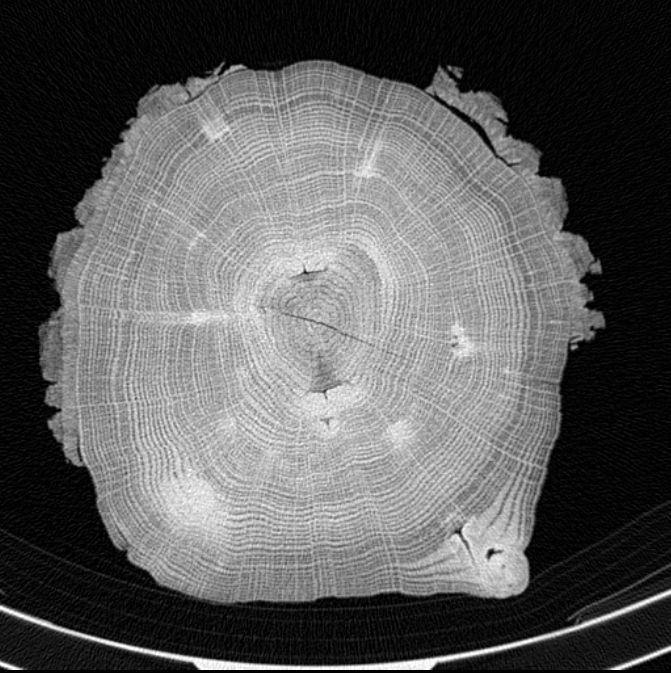
\includegraphics[width=\textwidth]{images/challenge_knot_rot_boundary.png}
        \caption{Incomplete bark and a vague boundary between the knot and the surrounding healthy wood.}
        \label{fig:challenge_a}
    \end{subfigure}
    \hfill
    \begin{subfigure}[b]{0.45\textwidth}
        \centering
        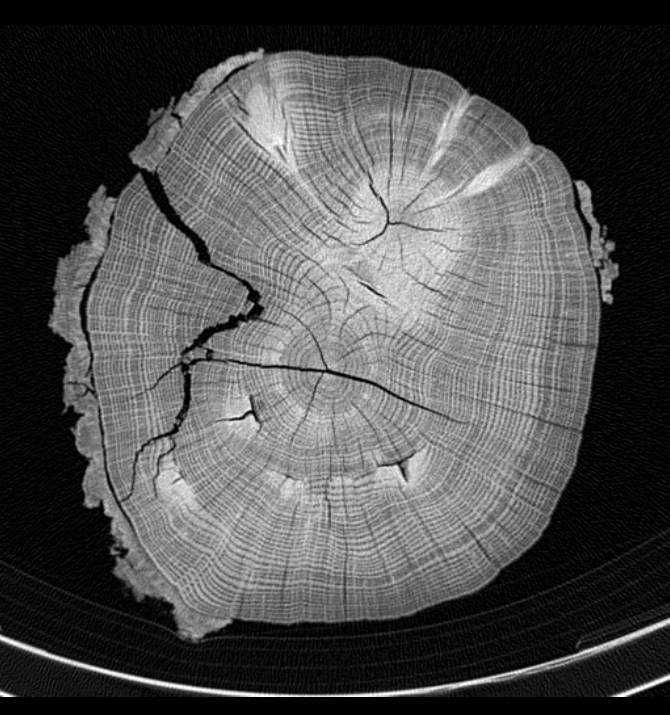
\includegraphics[width=\textwidth]{images/challenge_crack_rot.png}
        \caption{Incomplete bark, a thin crack and a thicker crack, and an elongated rot region.}
        \label{fig:challenge_b}
    \end{subfigure}

    \vskip\baselineskip

    \begin{subfigure}[b]{0.45\textwidth}
        \centering
        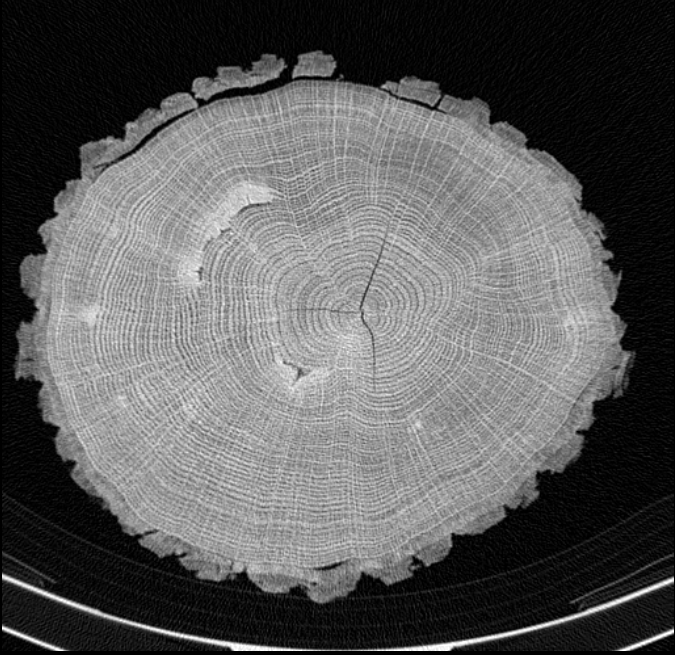
\includegraphics[width=\textwidth]{images/challenge_thin_crack.png}
        \caption{A thin crack and a thin elongated rot region.}
        \label{fig:challenge_c}
    \end{subfigure}
    \hfill
    \begin{subfigure}[b]{0.45\textwidth}
        \centering
        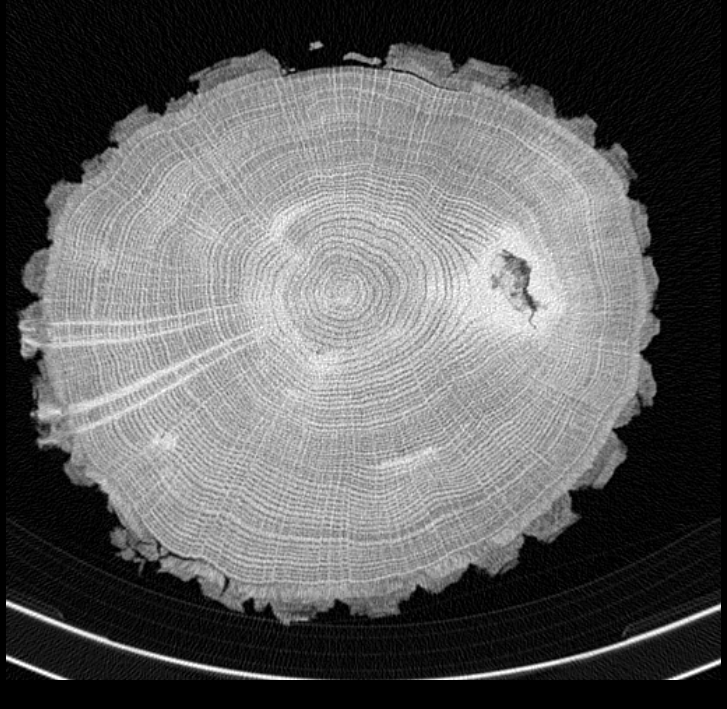
\includegraphics[width=\textwidth]{images/challenge_bark_boundary.png}
        \caption{Vague boundary between knot and rot.}
        \label{fig:challenge_d}
    \end{subfigure}
    \caption{Examples of annotation challenges in the dataset. Panels~(a) and~(b) show incomplete bark, with~(a) also illustrating an unclear knot to healthy wood transition and~(b) combining cracks of different widths with elongated rot. Panel~(c) shows a thin crack alongside a narrow rot region only a few voxels wide. Panel~(d) shows the gradient transition between knot and rot, where the boundary is a density gradient rather than a sharp edge.}
    \label{fig:annotation_challenges}
\end{figure}

Overall, the dataset presents four main challenges for modeling. These include strong class imbalance, small and irregular defect structures, high variability within each class, and spatial overlap between defects. As shown in Figure~\ref{fig:annotation_challenges}, boundaries between defects such as knots and rot are often unclear, cracks can be only a few voxels wide, and bark intensity varies locally. These factors should be addressed during training through sampling strategies, suitable loss functions, and models that can use spatial context.

\section{Data Split Strategy}

The six annotated logs were divided into three non-overlapping subsets, namely test, training, and validation.

A complete log volume, \textit{dub3}, was kept exclusively as a test set and was not used at any stage of training or hyperparameter selection. The remaining five logs (\textit{dub1}, \textit{dub2}, \textit{dub5}, \textit{dub11}, \textit{dub37}) were used to construct the training and validation sets.

Holding out a complete log rather than partitioning every volume reflects the goal of evaluating generalization across trees rather than across slices of the same tree. Slices within a single log are highly correlated, since neighboring slices differ by only one millimeter of wood, so a slicewise split would leak information across subsets. The voxel coverage of the test log \textit{dub3} is reported in Table~\ref{tab:test_coverage} and follows the same overall distribution as the training data described in Section~\ref{sec:dataset_characteristics}, which means that the test log is representative of the dataset as a whole.

\begin{table}[htbp]
    \centering
    \caption{Voxel count and class coverage in the test volume \textit{dub3}. The distribution closely matches the overall dataset characteristics reported in Section~\ref{sec:dataset_characteristics}.}
    \label{tab:test_coverage}
    \begin{tabular}{lrr}
        \toprule
        \textbf{Class} & \textbf{Voxels} & \textbf{Coverage} \\
        \midrule
        Background     & 59\,206\,176 & 45.17\,\% \\
        Healthy Wood   & 61\,022\,144 & 46.56\,\% \\
        Bark           &  6\,281\,039 &  4.79\,\% \\
        Knot           &  4\,431\,113 &  3.38\,\% \\
        Crack          &      64\,707 &  0.05\,\% \\
        Rot            &      60\,517 &  0.05\,\% \\
        Insect Damage  &       6\,304 &  $<$0.01\,\% \\
        \bottomrule
    \end{tabular}
\end{table}

To ensure a diverse validation set and prevent the model from overfitting to the specific morphology of a single tree, the five remaining logs were partitioned along the longitudinal axis into smaller sections. Each section contained roughly 300 CT slices, representing approximately 20~cm of wood. By dividing the logs into smaller items rather than relying on full volumes, the validation set could be constructed from multiple distinct trees, capturing a much wider variance of internal structural configurations.

This partitioning yielded a total of 20 partial volumes. The validation set was formed by selecting four distinct partial volumes, each originating from a different log, namely \textit{dub1part1}, \textit{dub5part2}, \textit{dub11part3}, and \textit{dub37part4}. The remaining 16 sections were used for training. The four sections of \textit{dub2} were assigned to the training set to maintain an approximate 75:25 split between training and validation, since the validation set already included four distinct sections of four different logs.

A cross-validation scheme was considered, but a single fixed split was used instead, prioritizing time and compute on hyperparameter and architecture tuning over repeated validation runs. Drawing the four validation sections from four different logs at four different spatial positions also partly compensates for the variability of a single fixed split.

\section{Model Selection}

The literature review in Chapter~\ref{chap:research} highlighted three observations relevant to this dataset. First, methods using full 3D context outperformed slicewise approaches when generalizing across wood species~\cite{Schmoldt_1998}. Second, slicewise convolutional networks struggled to represent intricate knot configurations, which motivated the use of self-attention~\cite{khazem2023deep}. Third, nnU-Net's adaptive configuration won the Medical Segmentation Decathlon on datasets with limited training data and severe class imbalance~\cite{isensee2021nnunet, antonelli2022msd}, characteristics the oak log dataset shares.

Therefore, three architectures were selected. nnU-Net~\cite{isensee2021nnunet} provides a strong convolutional reference. MedNeXt~\cite{roy2023mednext} extends the convolutional approach with large kernels that approximate the broad receptive fields of attention while preserving the convolutional inductive bias. SwinUNETR~\cite{hatamizadeh2022swinunetr} replaces the encoder with a hierarchical Swin Transformer that computes self-attention within shifted local windows, providing global context.

nnU-Net is also evaluated in its 2D, 3D full resolution and 3D cascade configurations to identify which configuration best fits the anisotropic voxel spacing and the defect scale distribution.

\section{Loss Function Selection}

The class imbalance shown in Figures~\ref{fig:barplot_coverage_pct} and~\ref{fig:barplot_coverage_pct_defects} dictates the choice of loss function. With background and healthy wood occupying roughly 93\,\% of the voxels and insect damage only 0.007\,\%, voxelwise losses such as cross-entropy place almost all weight on the dominant classes. Region overlap losses such as Dice~\cite{milletari2016vnet} address this by treating each class as a region and penalizing the predicted region's mismatch with the ground truth mask, independently of class size.

Cracks pose a second structural problem. They appear as long thin sheets that occupy a few voxels per slice but extend across many slices. A small offset in the prediction can leave the resulting crack disconnected from its true axis, which a region overlap loss only weakly penalizes. The skeleton recall term introduced by~\cite{kirchhoff2024skeletonrecall} explicitly rewards predictions that cover the medial axis of each foreground class.

The proposed loss combines three terms that target different aspects of the problem. Weighted cross-entropy operates at the voxel level and penalizes per-voxel misclassification with class-frequency weights. Soft Dice operates at the region level and penalizes mismatched class regions independently of their size. Skeleton recall operates at the topology level and penalizes predictions that fail to cover thin elongated structures.

Soft Dice~\cite{milletari2016vnet} optimizes the overlap between predicted and ground truth masks:

\begin{equation}
\mathcal{L}_{\text{Dice}} = 1 - \frac{2 \sum_i p_i g_i + \epsilon}{\sum_i p_i + \sum_i g_i + \epsilon}
\label{eq:dice}
\end{equation}

where $p_i$ and $g_i$ denote the predicted probability and ground truth value at voxel $i$, and $\epsilon$ is a smoothing constant.

Weighted cross-entropy reweights the standard cross-entropy by class frequency:

\begin{equation}
\mathcal{L}_{\text{CE}} = -\sum_i w_c \, g_i \log p_i
\label{eq:ce}
\end{equation}

where $w_c$ denotes the weight assigned to class $c$, set inversely proportional to the frequency of class $c$ in the training set.

The skeleton recall loss~\cite{kirchhoff2024skeletonrecall} measures whether the model recovers the medial axis of each foreground class:

\begin{equation}
\mathcal{L}_{\text{Skel}} = 1 - \frac{1}{|C_{\text{fg}}|} \sum_{c \in C_{\text{fg}}} \frac{\sum_i p_{i,c} \cdot s_{i,c}}{\sum_i s_{i,c} + \epsilon}
\label{eq:skel}
\end{equation}

where $s_{i,c}$ is the binary medial axis skeleton of the ground truth mask for class $c$, and $C_{\text{fg}}$ denotes the set of foreground classes. The skeleton is computed once using the 3D medial axis transform and treated as a constant during backpropagation.

The three terms are combined as follows:

\begin{equation}
\mathcal{L} = \mathcal{L}_{\text{CE}} + \mathcal{L}_{\text{Dice}} + \mathcal{L}_{\text{Skel}}
\label{eq:combined_loss}
\end{equation}

The background class was excluded from the Dice and skeleton terms to prevent its size from dominating the foreground classes.


\chapter{Training}

The training phase for the three architectures is described in this chapter. For all three models, namely nnU-Net, MedNeXt, and SwinUNETR, a manual selection of hyperparameters is presented. In addition, MedNeXt and SwinUNETR required a custom data augmentation pipeline.

\section{nnU-Net}

The nnU-Net baseline retained the framework's default training configuration, using SGD with Nesterov momentum and a polynomial learning rate schedule starting at $10^{-2}$. The patch size of $[224, 128, 224]$ voxels was set after splitting the original CT volumes into smaller sub-volumes for cross-validation, and the batch size remained at the framework's default of 2.

\subsection{Augmentation}

nnU-Net employs an automatically configured augmentation pipeline. This includes random rotations, scaling, axis flips, Gaussian noise, blurring, brightness and contrast adjustments, gamma corrections, and elastic deformations. The augmentation parameters are derived directly from the dataset fingerprint, which includes image size and voxel spacing, so that all transformations are appropriately scaled to the characteristics of the dataset.

\subsection{Training Dynamics}

Training and validation loss, along with the Pseudo Dice heuristic, were monitored to assess learning and overfitting.

Figure~\ref{fig:nnunet_training_curve} shows a rapid reduction in initial loss over 140 epochs. The training loss (blue) decreases smoothly, while the validation loss (red) is noticeably noisier and sits above the training loss for most of the run. This reflects the small validation set rather than instability in the model. With only four sections drawn from four different logs, each validation pass evaluates a tiny sample of the overall data distribution, so small shifts in which patches are sampled produce visible epoch to epoch variation. The EMA of the Pseudo Dice (green) smooths out this noise and converges to a plateau just below 0.82, indicating that the model has reached its learning capacity and justifying the choice to stop training.

\begin{figure}[H]
\centering
\includegraphics[width=0.95\textwidth]{images/training_curve_nnunet.png}
\caption{Training progression graph generated by the nnU-Net framework.}
\label{fig:nnunet_training_curve}
\end{figure}

\section{SwinUNETR}

SwinUNETR was trained using the AdamW optimizer~\cite{loshchilov2019adamw} with an initial learning rate of $10^{-3}$ and a weight decay of $10^{-4}$. AdamW was selected because it decouples weight decay from the adaptive gradient update, applying the regularization penalty directly to the weights rather than folding it into the gradient. This produces more consistent regularization than standard Adam with an $L_2$ penalty.

A linear warmup of 20 epochs was used at the start of training. The learning rate increased tenfold over this period, from $10^{-4}$ to the target value of $10^{-3}$, before the main training schedule took over. The warmup stabilizes the early gradient updates and prevents large parameter jumps before the network has adapted to the data distribution.

Training used 3D patches of size $224 \times 180 \times 224$ voxels. The axial dimensions of $224 \times 224$ match the square in plane shape of the CT scans, which measure $512 \times 512$ voxels in the axial plane. The longitudinal size of 180 voxels was set by GPU memory limits, since the available A100 with 40\,GB of VRAM did not allow a larger size and any increase above 180 caused out of memory errors during training. The batch size was 4 with gradient accumulation over 4 iterations, giving an effective batch size of 16. Gradient norms were clipped at 1.0 and a dropout rate of 0.2 was used to reduce overfitting.

\subsection{Augmentation}
\label{sec:custom_augmentation}

A custom augmentation pipeline was built using the MONAI~\cite{cardoso2022monai} library to address the severe class imbalance shown in Figures~\ref{fig:barplot_coverage_pct} and~\ref{fig:barplot_coverage_pct_defects}. The pipeline combines input normalization, class-balanced patch sampling, spatial transforms, photometric transforms, and coarse dropout. Each transform is applied online during training with a probability and parameter range chosen to preserve plausible wood geometry. The complete configuration is summarized in Table~\ref{tab:augmentation_pipeline}.

\begin{table}[htbp]
\centering
\caption{MONAI augmentation pipeline used for SwinUNETR and MedNeXt training. All probabilities and parameters apply per training sample. Sampling ratios in the bottom block are relative to the background rate of 1.0.}
\label{tab:augmentation_pipeline}
\small
\begin{tabular}{lll}
    \toprule
    \textbf{Stage} & \textbf{Transform} & \textbf{Parameters} \\
    \midrule
    Normalization & \texttt{ScaleIntensityRanged} & Clip to $[-1000, +500]$ HU \\
                  & \texttt{NormalizeIntensityd}  & Training set mean and std \\
    \midrule
    Spatial       & \texttt{RandFlipd}            & p = 0.5, axial axes only \\
                  & \texttt{Rand3DElasticd}       & p = 0.15, smoothness 5--6, magnitude 30--100 vox \\
                  & \texttt{RandAffined}          & p = 0.25, rotation $\pm 30^\circ$ around longitudinal axis, \\
                  &                               & translation 10 vox, scale $\pm 15$\,\% \\
    \midrule
    Photometric   & \texttt{RandHistogramShiftd}  & p = 0.15, 10 control points \\
                  & \texttt{RandGaussianNoised}   & p = 0.15, std 0.015 \\
                  & \texttt{RandAdjustContrastd}  & p = 0.15, gamma $[0.75, 1.4]$ \\
                  & \texttt{RandScaleIntensityd}  & p = 0.12, factor $\pm 8$\,\% \\
                  & \texttt{RandGaussianSmoothd}  & p = 0.08 \\
                  & \texttt{RandGaussianSharpend} & p = 0.08 \\
    \midrule
    Occlusion     & \texttt{RandCoarseDropoutd}   & p = 0.15, 5 holes of $16^3$ vox \\
    \midrule
    Sampling      & \texttt{RandCropByLabelClassesd} & Background 1.0, healthy wood 1.0, bark 2.0, \\
                  &                                  & knot 4.0, crack 5.0, rot 6.0, insect damage 8.0 \\
    \bottomrule
\end{tabular}
\end{table}

The spatial transforms exploit the approximate symmetry of oak logs around their longitudinal axis. Axial flips and rotation around this axis produce no implausible structures, so they are applied at high probability and with a wide angular range. Elastic deformation simulates natural grain variability. Photometric transforms simulate variability in scanner calibration, beam hardening, and reconstruction~\cite{bushberg2011essential}, which is relevant given that the dataset is drawn from a single scanner and the trained models should remain robust if applied to volumes from other scanners. Coarse dropout removes five random $16^3$ voxel regions per patch to encourage broader spatial context rather than reliance on localized features.

\subsubsection{Input Normalization}

All CT volumes were clipped to the range $[-1000, +500]$~HU to remove outliers and restrict the data to relevant wood densities~\cite{freyburger2009measuring}. Normalization was then performed using the mean and standard deviation calculated from the training set only and applied consistently to the training, validation, and test splits. This preserves absolute Hounsfield Unit relationships across logs and prevents the data leakage that would occur if the test split contributed to the normalization statistics.

\subsubsection{Class-Balanced Patch Sampling}

Initial sampling weights were estimated from the inverse square root of class coverage in Equation~\ref{eq:inverse_weight}, where $C_i$ denotes the voxel coverage of class $i$:

\begin{equation}
    W_i = \frac{1}{\sqrt{C_i}}
    \label{eq:inverse_weight}
\end{equation}

Direct use of these weights caused excessive oversampling of rare classes and overfitting to the few examples available in each. The weights were therefore scaled and capped to the final ratios reported in Table~\ref{tab:sampling_ratios}, which raise rare classes to between 2 and 8 times the background rate without forcing the model to memorize the small number of insect damage instances.

\begin{table}[htbp]
\centering
\caption{Comparison of class coverage, raw weights from the inverse square root formula, and final sampling ratios. Background and healthy wood were fixed at a baseline ratio of 1.0, while rare defect classes were scaled and capped to prevent overfitting.}
\label{tab:sampling_ratios}
\begin{tabular}{lrrr}
    \toprule
    \textbf{Class} & \textbf{Coverage (\%)} & \textbf{Weight Ratio ($W_i$)} & \textbf{Final Ratio} \\
    \midrule
    Background     & 45.66 & 0.15  & 1.0 \\
    Healthy Wood   & 47.12 & 0.15  & 1.0 \\
    Bark           &  4.78 & 0.46  & 2.0 \\
    Knot           &  1.52 & 0.81  & 4.0 \\
    Crack          &  0.77 & 1.14  & 5.0 \\
    Rot            &  0.14 & 2.64  & 6.0 \\
    Insect Damage  &  0.007 & 11.95 & 8.0 \\
    \bottomrule
\end{tabular}
\end{table}

\subsection{Training Dynamics}

Figure~\ref{fig:swinunetr_training_curve} shows loss and Dice over 113 epochs. Loss drops sharply in the first 20 epochs, then gradually converges. The validation loss remains slightly lower due to dropout and shows no overfitting.

The validation Dice rises rapidly until epoch 30 and plateaus, reaching a peak of 0.657 at epoch 110. The training to validation gap of roughly 0.78 against 0.62 reflects the difficulty of the task and the higher variance of transformer models on small datasets. Training stopped at 113 epochs after convergence.

\begin{figure}[H]
\centering
\begin{subfigure}[b]{0.48\textwidth}
\centering
\includegraphics[width=\textwidth]{images/swinunetr_loss.png}
\caption{Training and validation loss}
\end{subfigure}
\hfill
\begin{subfigure}[b]{0.48\textwidth}
\centering
\includegraphics[width=\textwidth]{images/swinunetr_dice.png}
\caption{Mean Dice coefficient}
\end{subfigure}
\caption{Training dynamics of the SwinUNETR model.}
\label{fig:swinunetr_training_curve}
\end{figure}

\subsection{Pretrained Weights}
\label{sec:pretrained_weights}

The self-supervised learning (SSL) pretrained backbone weights provided by MONAI (\texttt{model\_swinvit.pt})~\cite{tang2022swinunetrssl} were loaded via \texttt{model.load\_from()}. The encoder was initialized from these weights and the decoder and segmentation head were trained from scratch. The MONAI checkpoint was produced by pretraining the Swin Transformer encoder on a large unlabeled CT corpus using inpainting, contrastive learning, and rotation prediction objectives.

This initialization did not improve validation Dice or convergence compared to training from scratch. Despite the structural similarities at the CT level, the domain gap between medical anatomy and wood proved too large for meaningful feature transfer.

\section{MedNeXt}

MedNeXt was trained using the AdamW optimizer~\cite{loshchilov2019adamw} with the same learning rate, weight decay, and warmup schedule as SwinUNETR, namely an initial learning rate of $10^{-3}$, a weight decay of $10^{-4}$, and a 20 epoch linear warmup increasing the learning rate tenfold from $10^{-4}$ to $10^{-3}$. The patch size of $224 \times 180 \times 224$ voxels, the batch size of 4 with gradient accumulation over 4 iterations, the gradient clipping at 1.0, and the dropout rate of 0.2 were also retained from the SwinUNETR configuration.

\subsection{Augmentation}

MedNeXt used the same MONAI augmentation pipeline as SwinUNETR, described in Section~\ref{sec:custom_augmentation} and summarized in Table~\ref{tab:augmentation_pipeline}. Sharing the pipeline keeps the comparison between the two architectures fair, since any difference in performance reflects the architecture rather than the training data preparation.

\subsection{Pretrained Weights}

A custom trainer \texttt{nnUNetTrainerLungPretrained} was implemented to initialize encoder weights from a Lung CT segmentation checkpoint (Task006\_Lung). Lung CT was selected as the source domain because lung structures share some characteristics with the oak log volumes, including internal low density cavities and regions of varying density that produce comparable Hounsfield Unit contrasts. The segmentation head was retrained from scratch to match the output class count.

This initialization did not improve validation Dice or convergence compared to training from scratch, consistent with the SwinUNETR result reported in Section~\ref{sec:pretrained_weights}.

\subsection{Training Dynamics}

Figure~\ref{fig:mednext_training_curve} shows MedNeXt training over 168 epochs. The loss decreases rapidly, falling below 3.0 within 25 epochs, then more gradually, reaching 1.88 on the training set while the validation loss stabilizes around 2.0 without overfitting.

Validation Dice peaks at 0.697 at epoch 118 before slightly declining, indicating saturation. The smaller training to validation gap compared to SwinUNETR reflects the stronger inductive bias of the convolutional architecture. Training stopped at 168 epochs after performance plateaued.

\begin{figure}[H]
\centering
\begin{subfigure}[b]{0.48\textwidth}
\centering
\includegraphics[width=\textwidth]{images/mednext_loss.png}
\caption{Training and validation loss}
\end{subfigure}
\hfill
\begin{subfigure}[b]{0.48\textwidth}
\centering
\includegraphics[width=\textwidth]{images/mednext_dice.png}
\caption{Mean Dice coefficient}
\end{subfigure}
\caption{Training dynamics of the MedNeXt model.}
\label{fig:mednext_training_curve}
\end{figure}
\section{Postprocessing}

The trained models produce per voxel class predictions that contain systematic misclassifications caused by class combinations that are rare in the training data. Four rules are applied in sequence to the raw prediction mask. Each rule targets a failure identified through predictions from the validation set and the inter-class distance analysis in Figure~\ref{fig:distance_matrix}.

\begin{algorithm}[H]
\caption{Rule-based postprocessing of a predicted 3D label volume}
\label{alg:postprocess}
\begin{algorithmic}[1]
\Require Predicted label volume $P$ with classes: background, bark, healthy wood, crack, rot, knot, insect damage
\Ensure Corrected label volume $P'$
\State Dilate all crack voxels by $d_\text{rot-crack} = 2$\,px to obtain neighbourhood $N_\text{crack}$
\ForAll{connected components $R_i$ in rot mask}
  \If{any voxel of $R_i$ lies within $N_\text{crack}$}
    \State Relabel all voxels of $R_i$ as crack
  \EndIf
\EndFor
\State Dilate all bark voxels by $d_\text{crack-bark} = 10$\,px to obtain neighbourhood $N_\text{bark}$
\ForAll{connected components $C_j$ in crack mask}
  \If{$|C_j \cap N_\text{bark}| \,/\, |C_j| \;\geq\; 0.8$}
    \State Relabel all voxels of $C_j$ as background
  \EndIf
\EndFor
\State Dilate all rot voxels by $1$\,px to obtain neighbourhood $N_\text{rot}$
\ForAll{connected components $B_k$ in background mask}
  \If{$|B_k| < 50\,000$ and $B_k$ intersects $N_\text{rot}$}
    \State Relabel all voxels of $B_k$ as rot
  \EndIf
\EndFor
\ForAll{defect classes $d \in \{\text{knot, rot, bark, crack, insect}\}$}
  \State $F \gets$ masks of the filled holes from $\text{mask}(d)$ 
  \ForAll{connected components $H$ in $F \setminus \text{mask}(d)$ where label $\in \{\text{BG, HW}\}$ and $|H| \leq 50\,000$}
    \State Relabel all voxels of $H$ as $d$
  \EndFor
\EndFor
\State $P' \gets P$ with the relabeling applied
\end{algorithmic}
\end{algorithm}

Cracks that pass through knots are often classified as rot because most rot in the dataset
appears inside knots.
Only the ends of such cracks that lie outside the knot tend to be correctly classified.
If any voxel of a rot component lies within $2$\,px of a crack voxel, the whole component is
relabeled as crack.

\begin{figure}[H]
    \centering
    \begin{subfigure}[b]{0.48\textwidth}
        \centering
        \includegraphics[width=\textwidth, height=4.5cm]{images/pp_rot_crack_before.png}
        \caption{Rot inside a knot classified incorrectly}
        \label{fig:pp_rot_crack_before}
    \end{subfigure}
    \hfill
    \begin{subfigure}[b]{0.48\textwidth}
        \centering
        \includegraphics[width=\textwidth, height=4.5cm]{images/pp_rot_crack_after.png}
        \caption{After postprocessing}
        \label{fig:pp_rot_crack_after}
    \end{subfigure}
    \caption{Rule 1: a rot component that touches a crack voxel within
    2\,px~(a) is relabeled as crack~(b). This corrects errors inside knots.}
    \label{fig:pp_rot_crack}
\end{figure}

Predictions near the bark boundary sometimes produce thin crack fragments that lie almost
entirely within the bark neighborhood.
These fragments are artifacts on the boundary rather than real cracks.
Any crack component for which at least $80\,\%$ of its voxels are within $10$\,px of bark
is relabeled as background.

\begin{figure}[H]
    \centering
    \begin{subfigure}[b]{0.48\textwidth}
        \centering
        \includegraphics[width=\textwidth, height=4.5cm]{images/pp_crack_background_before.png}
        \caption{Crack near bark classified incorrectly}
        \label{fig:pp_crack_bg_before}
    \end{subfigure}
    \hfill
    \begin{subfigure}[b]{0.48\textwidth}
        \centering
        \includegraphics[width=\textwidth, height=4.5cm]{images/pp_crack_background_after.png}
        \caption{After postprocessing}
        \label{fig:pp_crack_bg_after}
    \end{subfigure}
    \caption{Rule 2: a crack component with ${\geq}\,80\,\%$ of its
    voxels within 10\,px of bark~(a) is relabeled as background~(b). This removes
    artifacts at the boundary.}
    \label{fig:pp_crack_bg}
\end{figure}

Dense dark rot regions are visually similar to air and are sometimes classified as
background.
Any background component smaller than $50\,000$\,voxels that lies next to rot is relabeled as rot.
The size threshold ensures that the outer background is not affected.

\begin{figure}[H]
    \centering
    \begin{subfigure}[b]{0.48\textwidth}
        \centering
        \includegraphics[width=\textwidth, height=4.5cm]{images/pp_background_rot_before.png}
        \caption{Misclassified background inside rot}
        \label{fig:pp_bg_rot_before}
    \end{subfigure}
    \hfill
    \begin{subfigure}[b]{0.48\textwidth}
        \centering
        \includegraphics[width=\textwidth, height=4.5cm]{images/pp_background_rot_after.png}
        \caption{After postprocessing}
        \label{fig:pp_bg_rot_after}
    \end{subfigure}
    \caption{Rule 3: a background component smaller than $50\,000$\,voxels that is next to rot~(a) is relabeled as rot~(b). This recovers dense regions of rot.}
    \label{fig:pp_bg_rot}
\end{figure}

Small pockets of healthy wood or background that are fully enclosed by a defect are voids that the model misidentifies. For each defect class, \texttt{scipy} binary hole filling is applied to each slice of that defect mask. Any resulting hole voxel that carries a healthy wood or background label and belongs to a connected component smaller than $50\,000$\,voxels are relabeled to the enclosing defect. This directly fills misclassified cavities.

\begin{figure}[H]
    \centering
    \begin{subfigure}[b]{0.48\textwidth}
        \centering
        \includegraphics[width=\textwidth, height=4.5cm]{images/pp_enclosed_before.png}
        \caption{Pocket enclosed by a knot}
        \label{fig:pp_enclosed_before}
    \end{subfigure}
    \hfill
    \begin{subfigure}[b]{0.48\textwidth}
        \centering
        \includegraphics[width=\textwidth, height=4.5cm]{images/pp_enclosed_after.png}
        \caption{After postprocessing}
        \label{fig:pp_enclosed_after}
    \end{subfigure}
    \caption{Rule 4: a healthy wood or background pocket fully enclosed by a defect~(a) is relabelled to the surrounding defect class~(b).
    This recovers internal voids incorrectly segmented by the model.}
    \label{fig:pp_enclosed}
\end{figure}


\chapter{Results}
\label{chap:results}

All three models were evaluated on the test log \textit{dub3} using Dice coefficient and IoU as primary metrics. The foreground mean excludes the background class and reflects the performance of the defect categories.

% \section{Training Dynamics and Convergence}

% The learning behavior of the model is evaluated using loss trends, convergence speed, and generalization performance. The analysis highlights training stability, identifies saturation points, and reveals differences in how effectively each architecture adapts to the dataset.

% \section{nnU-Net Configuration Selection}
% \label{sec:nnunet_config}

% nnU-Net offers three configurations for 3D segmentation tasks, namely 2D, 3D full resolution, and 3D cascade full resolution. All three were trained on the oak log dataset under the framework's default setting and compared on the validation set using the pseudo Dice metric reported during training.

% \begin{table}[H]
%     \centering
%     \caption{Validation pseudo Dice for the three nnU-Net configurations.}
%     \label{tab:nnunet_config}
%     \begin{tabular}{lc}
%         \toprule
%         \textbf{Configuration} & \textbf{Validation Pseudo Dice} \\
%         \midrule
%         2D                          & 0.73 \\
%         3D full resolution          & 0.79 \\
%         3D cascade full resolution  & \textbf{0.81} \\
%         \bottomrule
%     \end{tabular}
% \end{table}

% The 3D cascade full resolution configuration achieved the highest validation pseudo Dice and was selected as the nnU-Net baseline for the remainder of the experiments. The cascade processes the volume in two stages, where a low resolution pass produces an initial segmentation that is then refined at full resolution. This suits a dataset where defects span a wide range of scales, since the low resolution stage captures global context, while the full resolution stage recovers fine boundaries.


% \subsection{nnU-Net}

% Training and validation loss, along with the Pseudo Dice heuristic, were monitored to assess learning and overfitting.

% Figure~\ref{fig:nnunet_training_curve} shows a rapid reduction in initial loss over 140 epochs. The training loss (blue) decreases smoothly, while the validation loss (red) is noticeably noisier and sits above the training loss for most of the run. This reflects the small validation set rather than the instability in the model. With only four sections drawn from four different logs, each validation pass evaluates a tiny sample of the overall data distribution, so small shifts in which patches are sampled produce visible epoch to epoch variation. The EMA of the Pseudo Dice (green) smooths out this noise and converges to a plateau just below 0.82, indicating that the model has reached its learning capacity and justifying the choice to stop training.

% \begin{figure}[H]
% \centering
% \includegraphics[width=0.95\textwidth]{images/training_curve_nnunet.png}
% \caption{Training progression graph generated by the nnU-Net framework.}
% \label{fig:nnunet_training_curve}
% \end{figure}

% \subsection{SwinUNETR}

% Figure~\ref{fig:swinunetr_training_curve} shows loss and Dice over 113 epochs. Loss drops sharply in the first 20 epochs, then gradually converges. The validation loss remains slightly lower due to dropout and shows no overfitting.

% The validation dice rises rapidly until epoch 30 and plateaus, reaching a peak of 0.657 (epoch 110). The train–validation gap (~0.78 vs. ~0.62) reflects the difficulty of the task and the higher variance of the transformer models in small datasets. Training stopped at 113 epochs after convergence.

% \begin{figure}[H]
% \centering
% \begin{subfigure}[b]{0.48\textwidth}
% \centering
% \includegraphics[width=\textwidth]{images/swinunetr_loss.png}
% \caption{Training and validation loss}
% \end{subfigure}
% \hfill
% \begin{subfigure}[b]{0.48\textwidth}
% \centering
% \includegraphics[width=\textwidth]{images/swinunetr_dice.png}
% \caption{Mean Dice coefficient}
% \end{subfigure}
% \caption{Training dynamics of the SwinUNETR model.}
% \label{fig:swinunetr_training_curve}
% \end{figure}

% \subsection{MedNeXt}

% Figure~\ref{fig:mednext_training_curve} shows MedNeXt training over 168 epochs. The loss decreases rapidly (below 3.0 within 25 epochs), then gradually, reaching 1.88 (training) while the validation stabilizes around 2.0 without overfitting.

% Validation Dice peaks at 0.697 (epoch 118) before slightly declining, indicating saturation. The smaller train–validation gap compared to SwinUNETR reflects a stronger inductive bias. Training stopped at 168 epochs after performance plateaued.

% \begin{figure}[H]
% \centering
% \begin{subfigure}[b]{0.48\textwidth}
% \centering
% \includegraphics[width=\textwidth]{images/mednext_loss.png}
% \caption{Training and validation loss}
% \end{subfigure}
% \hfill
% \begin{subfigure}[b]{0.48\textwidth}
% \centering
% \includegraphics[width=\textwidth]{images/mednext_dice.png}
% \caption{Mean Dice coefficient}
% \end{subfigure}
% \caption{Training dynamics of the MedNeXt model.}
% \label{fig:mednext_training_curve}
% \end{figure}

\section{Overall Segmentation Performance}

Table~\ref{tab:overall_results} summarizes the mean Dice and IoU for each model after postprocessing. nnU-Net achieves the highest overall scores, followed by MedNeXt and SwinUNETR.

\begin{table}[H]
    \centering
    \caption{Overall segmentation performance on the test log \textit{dub3} after postprocessing. The mean is computed over all foreground classes.}
    \label{tab:overall_results}
    \begin{tabular}{lcc}
        \toprule
        \textbf{Model} & \textbf{Foreground Mean Dice} & \textbf{Foreground Mean IoU} \\
        \midrule
        nnU-Net    & \textbf{0.833} & \textbf{0.724} \\
        MedNeXt    & 0.783          & 0.656          \\
        SwinUNETR  & 0.756          & 0.613          \\
        \bottomrule
    \end{tabular}
\end{table}

After postprocessing, nnU-Net leads all models. The gap over MedNeXt is 0.050 Dice and over SwinUNETR is 0.077. The relatively small dataset likely disadvantages the transformer architecture, which relies on more data to learn global dependencies.

\section{Per-Class Analysis}

Table~\ref{tab:perclass_results} reports per-class Dice for all three models. Healthy Wood achieves the highest scores across the board, as it constitutes the dominant volume and is geometrically simple. Bark scores are consistently high, but slightly lower due to irregular surface geometry and low contrast at the log boundary.

\begin{table}[H]
    \centering
    \caption{Per-class Dice on the test log \textit{dub3} after postprocessing. Bold values indicate the best score per class.}
    \label{tab:perclass_results}
    \begin{tabular}{lccc}
        \toprule
        \textbf{Class} & \textbf{nnU-Net} & \textbf{MedNeXt} & \textbf{SwinUNETR} \\
        \midrule
        Healthy Wood  & \textbf{0.981} & 0.966 & 0.885 \\
        Knot          & \textbf{0.808} & 0.665 & 0.706 \\
        Rot           & \textbf{0.864} & 0.832 & 0.683 \\
        Bark          & \textbf{0.861} & 0.819 & 0.814 \\
        Crack         & \textbf{0.794} & 0.759 & 0.762 \\
        Insect Damage & \textbf{0.691} & 0.654 & 0.683 \\
        \midrule
        \textbf{Mean} & \textbf{0.833} & 0.783 & 0.756 \\
        \bottomrule
    \end{tabular}
\end{table}

nnU-Net leads all classes, but several margins are narrow. Healthy wood and bark remain the highest scoring classes for all three models, reflecting their large extent and clearer textural separation. Knot is the lowest scoring class for both nnU-Net and MedNeXt, consistent with the gradual HU transition between dense knot tissue and the surrounding wood. Insect damage is the lowest scoring class for SwinUNETR and MedNeXt, and the second lowest for nnU-Net, where it ties almost exactly with SwinUNETR (0.691 against 0.683). Across the architectures, the smallest and most sparsely distributed classes consistently produce the lowest Dice values regardless of which model is used.

\section{Confusion Matrix}

Table~\ref{tab:cmnnunet} shows the row-normalised confusion matrix for nnU-Net on the test log \textit{dub3}. Each row is a true class and each column a predicted class; values are percentages of voxels in that true class.

\begin{table}[H]
    \centering
    \caption{Row-normalised confusion matrix for nnU-Net on the test log \textit{dub3}. Values are percentages of each true class. Bold diagonal entries show correctly classified voxels. BG stands for background and HW stands for healthy wood.}
    \label{tab:cmnnunet}
    \begin{adjustbox}{max width=\textwidth}
    \begin{tabular}{lrrrrrrr}
        \toprule
        & \textbf{BG} & \textbf{HW} & \textbf{Knot} & \textbf{Rot} & \textbf{Bark} & \textbf{Crack} & \textbf{Insect} \\
        \midrule
        BG     & \textbf{98.0} &  0.0 &  0.0 &  0.0 &  2.0 & 0.0 & 0.0 \\
        HW     &  0.0 & \textbf{98.1} &  0.7 &  0.0 &  1.1 & 0.0 & 0.0 \\
        Knot   &  0.0 & 25.5 & \textbf{74.3} &  0.2 &  0.0 & 0.0 & 0.0 \\
        Rot    &  0.0 &  0.1 & 10.4 & \textbf{89.5} &  0.0 & 0.0 & 0.0 \\
        Bark   &  1.0 &  0.7 &  0.0 &  0.0 & \textbf{98.4} & 0.0 & 0.0 \\
        Crack  &  0.0 &  6.1 &  0.0 &  0.0 &  0.0 & \textbf{93.9} & 0.0 \\
        Insect &  0.3 & 19.1 &  0.0 &  0.0 &  7.3 & 0.0 & \textbf{73.4} \\
        \bottomrule
    \end{tabular}
    \end{adjustbox}
\end{table}

Background and healthy wood achieve high recall (99.0\,\% and 98.2\,\%). Knot has the lowest recall at 70.0\,\%, with 29.8\,\% of knot voxels predicted as healthy wood, reflecting the gradual HU transition between dense knot tissue and the surrounding wood. Rot reaches 84.5\,\%, with 12.3\,\% confused with knot due to overlapping HU ranges in decayed tissue. Bark and crack are well separated at 93.8\,\% and 92.5\,\%. Insect damage scores 76.1\,\%, with 18.0\,\% misclassified as healthy wood, consistent with its small volume and sparse distribution. A smaller pattern is the mutual confusion at the bark boundary, where bark leaks 5.3\,\% to background and 0.9\,\% to healthy wood, while healthy wood leaks 1.2\,\% to bark. These errors concentrate at the log surface, where contrast between bark and the layers immediately on either side is low.


\section{Effect of Postprocessing}

Table~\ref{tab:postprocessing_results} shows the foreground mean Dice before and after postprocessing for each model.
\begin{table}[H]
    \centering
    \caption{Foreground mean Dice before and after postprocessing on the test log \textit{dub3}.}
    \label{tab:postprocessing_results}
    \begin{tabular}{lcc}
        \toprule
        \textbf{Model} & \textbf{Before} & \textbf{After} \\
        \midrule
        nnU-Net   & 0.775 & \textbf{0.833} \\
        MedNeXt   & 0.744 & 0.783 \\
        SwinUNETR & 0.702 & 0.756 \\
        \bottomrule
    \end{tabular}
\end{table}
Postprocessing affects mainly rot and crack because the four rules in Algorithm~\ref{alg:postprocess} relabel between rot, crack, background, and healthy wood pockets enclosed by defects. The largest single gain was on crack for nnU-Net, which rose from 0.446 to 0.794 and moved this class from the weakest to one of the stronger ones for that model. The other two models also gained substantially on crack, with SwinUNETR rising by 0.282 and MedNeXt by 0.149. MedNeXt benefited most on rot, where Rule 3 recovered dense regions that had been classified as background. For nnU-Net the rot score did not improve, with a marginal change of $-0.001$ Dice. The aggregate effect on foreground mean Dice was 0.058 for nnU-Net, 0.054 for SwinUNETR, and 0.039 for MedNeXt.
\section{Representative Predictions}
Figure~\ref{fig:qualitative_comparison} presents axial slices from the test log \textit{dub3}, with the ground truth displayed in the left column and the nnU-Net predictions in the right column. The ground truth column specifies which classes are present, while the prediction column indicates which classes were misclassified and which were correctly identified.

\begin{figure}[p]
    \centering

    % Row 1 -- good: knot
    \begin{subfigure}[b]{0.47\textwidth}
        \centering
        \includegraphics[width=\textwidth]{images/pred1gt.png}
        \caption{Ground truth: Healthy wood, Bark, Crack, Knot, Rot}
        \label{fig:row1_gt}
    \end{subfigure}
    \hfill
    \begin{subfigure}[b]{0.47\textwidth}
        \centering
        \includegraphics[width=\textwidth]{images/pred1.png}
        \caption{Accurate: Bark, Crack, Knot; Inaccurate: Healthy wood, Rot}
        \label{fig:row1_pred}
    \end{subfigure}

    \vskip\baselineskip

    % Row 2 -- good: rot
    \begin{subfigure}[b]{0.47\textwidth}
        \centering
        \includegraphics[width=\textwidth]{images/pred2gt.png}
        \caption{Ground truth: Healthy wood, Bark, Crack, Knot, Rot, Insect damage}
        \label{fig:row2_gt}
    \end{subfigure}
    \hfill
    \begin{subfigure}[b]{0.47\textwidth}
        \centering
        \includegraphics[width=\textwidth]{images/pred2.png}
        \caption{Accurate: Bark, Crack, Insect damage; Inaccurate: Healthy wood, Knot, Rot}
        \label{fig:row2_pred}
    \end{subfigure}

    \vskip\baselineskip

    % Row 3 -- good: bark
    \begin{subfigure}[b]{0.47\textwidth}
        \centering
        \includegraphics[width=\textwidth]{images/pred7gt.png}
        \caption{Ground truth: Healthy wood, Bark, Crack, Knot, Rot, Insect damage}
        \label{fig:row3_gt}
    \end{subfigure}
    \hfill
    \begin{subfigure}[b]{0.47\textwidth}
        \centering
        \includegraphics[width=\textwidth]{images/pred7.png}
                \caption{Accurate: Knot, Rot; Inaccurate: Healthy wood, Bark, Crack, Insect damage}
        \label{fig:row3_pred}
    \end{subfigure}
    
  \caption{In (b), Rot is overestimated where tree rings are incorrectly identified. In (d), the central knot is not detected and is classified as healthy wood. The rot boundaries are slightly smaller than in the ground truth. In (f), a region of bark at the bottom is classified as healthy wood. The insect damage appears more elongated than expected, and the predicted crack is slightly larger than in the ground truth.}
  \label{fig:qualitative_comparison}
\end{figure}

\begin{figure}[p]
    \ContinuedFloat
    \centering

    % Row 4 -- failure: knot confused with healthy wood
    \begin{subfigure}[b]{0.47\textwidth}
        \centering
        \includegraphics[width=\textwidth]{images/pred4gt.png}
        \caption{Ground truth: Healthy wood, Bark, Crack, Knot}
        \label{fig:row4_gt}
    \end{subfigure}
    \hfill
    \begin{subfigure}[b]{0.47\textwidth}
        \centering
        \includegraphics[width=\textwidth]{images/pred4.png}
          \caption{Accurate: Bark, Crack; Inaccurate: Healthy wood, Knot}
        \label{fig:row4_pred}
    \end{subfigure}

    \vskip\baselineskip

    % Row 5 -- failure: insect damage missed
    \begin{subfigure}[b]{0.47\textwidth}
        \centering
        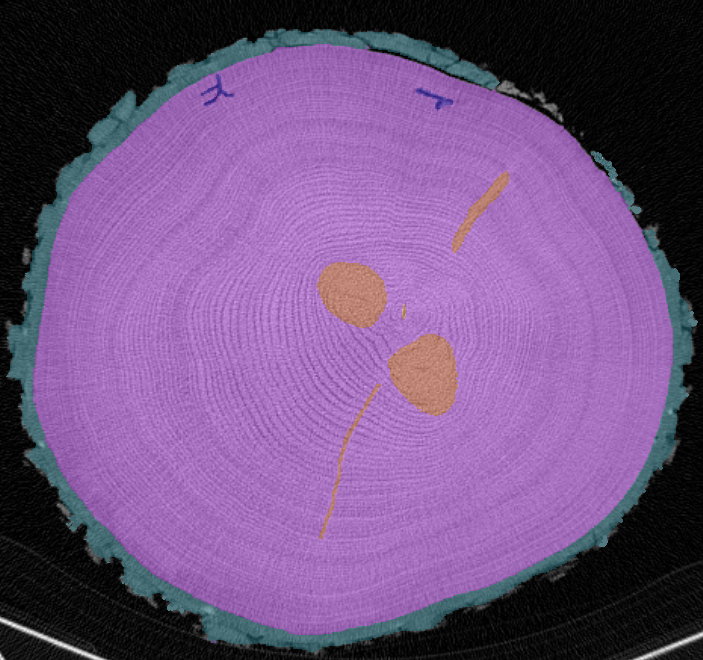
\includegraphics[width=\textwidth]{images/pred5gt.png}
        \caption{Ground truth: Healthy wood, Bark, Crack, Knot, Insect damage}
        \label{fig:row5_gt}
    \end{subfigure}
    \hfill
    \begin{subfigure}[b]{0.47\textwidth}
        \centering
        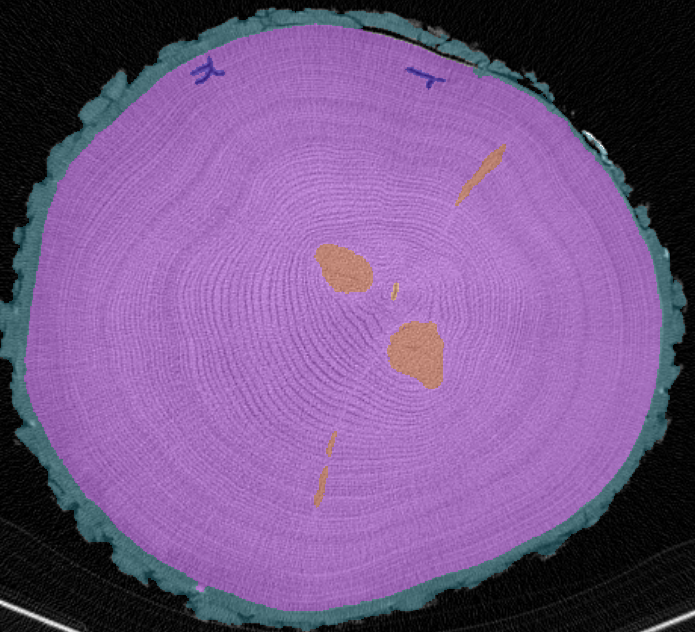
\includegraphics[width=\textwidth]{images/pred5.png}
        \caption{Accurate: Bark, Crack, Insect damage; Inaccurate: Healthy wood, Knot}
        \label{fig:row5_pred}
    \end{subfigure}

    \vskip\baselineskip

    % Row 6 -- failure: rot/knot confusion
    \begin{subfigure}[b]{0.47\textwidth}
        \centering
        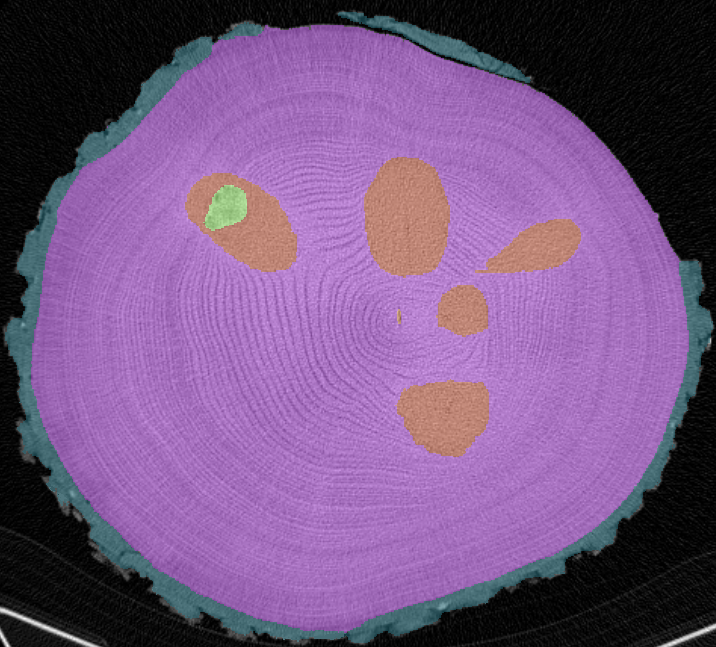
\includegraphics[width=\textwidth]{images/pred6gt.png}
        \caption{Ground truth: Healthy wood, Bark, Crack, Knot, Insect damage}
        \label{fig:row6_gt}
    \end{subfigure}
    \hfill
    \begin{subfigure}[b]{0.47\textwidth}
        \centering
        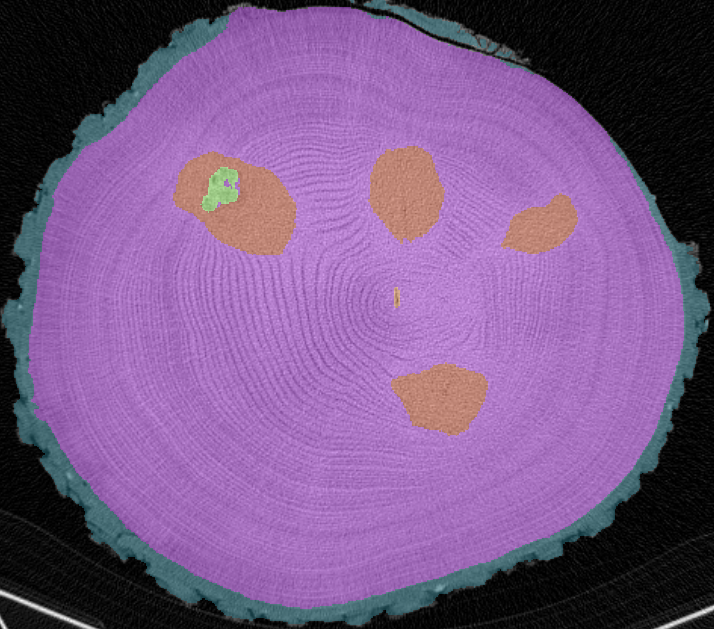
\includegraphics[width=\textwidth]{images/pred6.png}
        \caption{Accurate: Bark, Crack, Insect damage; Inaccurate: Healthy wood, Knot, Rot}
        \label{fig:row6_pred}
    \end{subfigure}

  \caption{In (h), a knot above the crack is not detected and the other knot boundaries are also inaccurate. In (j), the lower elongated knot is missing its upper portion. In (l), the rot boundaries are slightly inaccurate and a central knot is missing.}
\end{figure}

\chapter{Discussion}

\section{Architecture Comparison}

Table~\ref{tab:overall_results} places nnU-Net ahead of both MedNeXt and SwinUNETR on every aggregate metric, and Table~\ref{tab:perclass_results} confirms that the lead is consistent across classes after postprocessing. The 3D cascade configuration likely contributed the most to this result. The low resolution stage processes the entire volume at once and captures global context such as the position of a defect within the log and the overall shape of larger structures like rot regions or knot clusters. The full resolution stage then refines these predictions with localized detail, recovering thin cracks and sharp boundaries. This combination is well suited to a dataset where defects span a wide range of scales, from a few voxels of insect damage to centimeter scale rot.

SwinUNETR finished last with a foreground mean Dice of 0.756. The shifted window attention that defines the architecture is data hungry, and the persistent gap of roughly 0.16 between training and validation Dice indicates that the encoder did not see enough volumes to learn stable global dependencies. Transformers reward scale and 16 training sections do not deliver it. This is consistent with the Medical Segmentation Decathlon~\cite{antonelli2022msd}, where transformer variants tended to lag behind well configured CNNs on smaller tasks. The architecture is not a poor fit for volumetric wood defect segmentation in principle, it is a poor fit for the size of the corpus available here.

MedNeXt landed between the two, trailing nnU-Net by 0.050 Dice and leading SwinUNETR by 0.027. The large depthwise kernels that define this network were intended to approximate the broad receptive fields of attention while keeping the convolutional inductive bias intact. On this dataset they appear slightly oversized. The wider receptive field carries more parameters than the smaller convolutions in nnU-Net, and 16 training sections do not fully utilize that extra capacity. The per-class breakdown in Table~\ref{tab:perclass_results} is also more divided than the aggregate suggests. MedNeXt beats SwinUNETR on classes that are locally distinguishable by texture and density, namely healthy wood, rot, and bark, but loses on classes whose boundaries depend more on long range context such as knot, crack, and insect damage, where transformer attention apparently helps more than enlarged convolutions.

\section{Annotation and Class Ambiguity}

Several class boundaries in CT volumes are inherently ambiguous, and this same ambiguity was the dominant difficulty during manual annotation. Knot tissue fades gradually into surrounding healthy wood. Rot fades into knot. Bark blends into healthy wood on the inside and into background on the outside. These transitions are gradient regions rather than sharp edges, and even two human annotators tend to draw the boundary slightly differently.

The confusion matrix in Table~\ref{tab:cmnnunet} shows the same pattern in the prediction of the model. 29.8\,\% of knot voxels are predicted as healthy wood, 12.3\,\% of rot voxels are predicted as knot, and the bark boundary leaks in three directions at once (5.3\,\% bark to background, 0.9\,\% bark to healthy wood, and 1.2\,\% healthy wood to bark). These are not arbitrary errors. They sit on the same boundaries that made annotation difficult.

Bark is a useful reference point.~\cite{gergel2026wood} reported a bark Dice of 0.75 only after dedicated postprocessing. Bark in this work reaches 0.861 without any class specific rule, which suggests that 3D context and a more diverse training set help. The boundary errors that remain are likely amplified by suboptimal annotations.

\section{Dataset Limitations}

The annotated dataset covers six oak logs from a single scanning protocol, with a single log held out as the test set. The reported metrics therefore describe behavior on one specimen rather than on a population. A test set spanning more than one log would give a more reliable view of generalization across trees, but enlarging the test set further would have left an already small training and validation pool too thin to support three separate architectures within the available time.

All material is oak. Generalization to other species, log diameters, or scanners has not been tested and would require a separate evaluation.

Insect damage occupies 0.007\,\% of all voxels and remains the rarest class by a wide margin. Its Dice score is computed on a small number of voxels in a single test log and should be read as indicative rather than conclusive.

\chapter*{Conclusion}\addcontentsline{toc}{chapter}{Conclusion}\markboth{Conclusion}{Conclusion}

This thesis addressed the detection and classification of defects in oak logs scanned by computed tomography. All six tasks defined in the assignment were completed.

The literature review (Chapter~\ref{chap:research}) covered both the methodological landscape of CT based wood defect analysis and the available datasets. It established that prior work depends almost exclusively on private corpora, that 2D slicewise approaches dominate, and that no publicly available 3D annotated dataset of oak logs exists.

The defective categories were defined according to ČSN~EN~1310 and ČSN~EN~1311 (Section~\ref{sec:label_selection}). Four defect classes were selected, namely cracks, knots, rot, and insect damage. Bark was added as a structural class because separating it from the log interior is necessary to recover the usable wood volume.

A complete annotation methodology was designed and executed (Chapter~\ref{chap:dataset_annotation} and~\ref{sec:cvat_workflow}). Six logs were selected from the forty available, four of them with high defect density and two comparatively healthy. Background and bark masks were generated automatically using Otsu thresholding and SLIC superpixel clustering, which provided initial templates for the CVAT annotation pipeline. Defects inside the logs were annotated manually with the help of SAM based propagation between slices. The final corpus contains 6\,230 annotated CT slices.

The detection and classification algorithm builds on three 3D semantic segmentation architectures, namely nnU-Net, MedNeXt, and SwinUNETR. A custom loss combining Dice, weighted cross-entropy, and skeleton recall was used to handle class imbalance and the topology of thin elongated structures such as cracks. Four rule based postprocessing steps were derived from the class distance analysis to correct systematic misclassifications.

Results on the test log \textit{dub3} are reported in Chapter~\ref{chap:results}. The 3D cascade nnU-Net achieved the best foreground mean Dice of 0.833, followed by MedNeXt at 0.783 and SwinUNETR at 0.756. Postprocessing improved every model, with the largest gain on cracks. A row-normalized confusion matrix and per class Dice values describe the remaining error modes, most of which concentrate on the gradient transitions between knot, rot, and the surrounding wood.

Visualizations of the predictions are provided alongside the results. These confirm that the model recovers the major structural features of the log and most defects, with residual errors concentrated on small or sparsely distributed targets.

The dataset, the annotation pipeline, and the trained models together form a foundation for a system that informs sawmill cutting strategies. Future work includes scanning a larger and more diverse set of logs, extending the annotation effort beyond oak, and integrating the segmentation output with cutting plan optimization to translate voxel level predictions into measurable yield gains.